\begin{figure}[H]
	\centering
	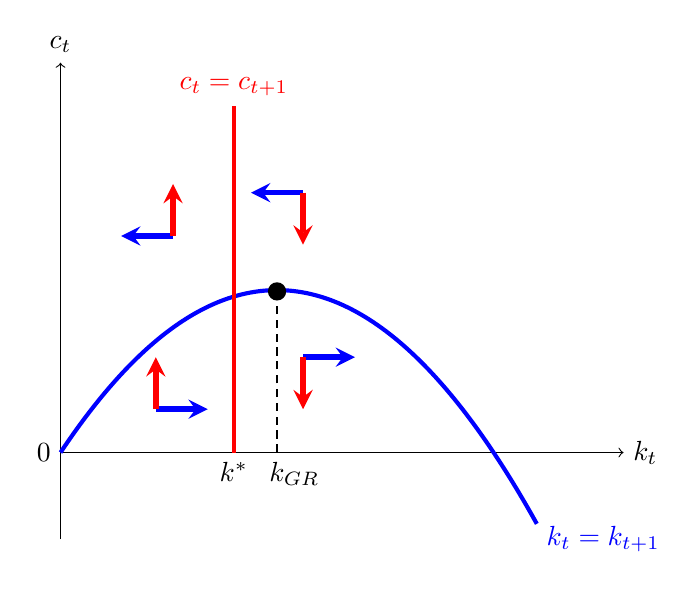
\begin{tikzpicture}[scale=1.1]
            \draw[->] (0, 0) -- (6.5, 0) node[right] {$k_{t}$};
            \draw[->] (0, -1) -- (0, 4.5) node[above] {$c_{t}$};
            % steady-state curves
            \draw[domain=0:5.5, samples=200, blue, line width=1.5pt, variable=\x] plot ({\x}, {-0.3*\x*(\x-5)});
            \draw[red, line width=1.5pt] (2,0) -- (2,4);
            \node[above] at (2,4) {\color{red}$c_{t} = c_{t+1}$};
            \node[right] at (5.5,-1) {\color{blue}$k_t = k_{t+1}$};
            % arrows depicting dynamics
            \draw[-stealth, blue, line width=2pt] (1.1,0.5) -- (1.7,0.5);
            \draw[-stealth, blue, line width=2pt] (2.8,3) -- (2.2,3);
            \draw[-stealth, blue, line width=2pt] (1.3,2.5) -- (0.7,2.5);
            \draw[-stealth, blue, line width=2pt] (2.8,1.1) -- (3.4,1.1);
            \draw[-stealth, red, line width=2pt] (2.8,3) -- (2.8,2.4);
            \draw[-stealth, red, line width=2pt] (1.3,2.5) -- (1.3,3.1);
            \draw[-stealth, red, line width=2pt] (1.1,0.5) -- (1.1,1.1);
            \draw[-stealth, red, line width=2pt] (2.8,1.1) -- (2.8,0.5);
            \draw[densely dashed, line width=1pt] (2.5,0) -- (2.5,1.86);
            % important nodes
            \node[left] at (0,-0) {$0$};
            \node[below] at (2,0) {$k^*$};
            \node[below] at (2.7,0) {$k_{GR}$};
            \fill[black] (2.5,1.86) circle (3pt);
	\end{tikzpicture}
\end{figure}
